\newcommand{\s}[1]{
    \(\mathcal{#1}\)}

\chapter{Metodologie}

\section{Formalizarea problemei}

Fie programul \s{P} un proiect Java, format dintr-o multime de fisere
clasa.  Scopul optimizatorului este sa creeze un program \s{P'}, care
sa se comporte identic cu \s{P}, si sa fie mai bun decat
\s{P} pentru o anumita metrica \s{M}.

\section{Diferentierea programelor}

Doua programe \s{P} si \s{Q} pot fi diferentiate daca
exista un input \s{I} pentru care \s{P} rulat pe \s{I}
si \s{Q} rulat pe \s{I} dau rezultate diferite.

\(\exists \mathcal{I}\) pentru care \(\mathcal{P}(\mathcal{I}) \ne
\mathcal{Q}(\mathcal{I}) \)

Unde prin rezultat intelegem atat output-ul programului, in
sensul pur matematic, cat si efectele laterale generate, care au
efect asupra mediului unde ruleaza programul.

Daca doua programe nu pot fi diferentiate (i.e., pentru toate
input-urile \s{I}, cele doua programe se comporta la fel), vom
spune despre ele ca sunt echivalente.

De exemplu, fie \s{P}

\begin{lstlisting}[language=Python,label={programul_p}]
def P(a: int, b: int) -> int:
    for i = 1:b
        a = inc(a)
    return a
\end{lstlisting}

si fie \s{Q}

\begin{lstlisting}[language=Python,label={programul_q}]
def Q(a: int, b: int) -> int:
    return a + b
\end{lstlisting}

atunci pentru orice a si b din $\N$, \s{P}(a, b) va fi egal cu
\s{Q}(a, b).

\section{Metrici de optimizare}

In contextul optimizarii de programe este nevoie sa definim ce
inseamn ca dintre doua programe echivalente \s{P} si \s{Q}, \s{P}
sa fie mai performant decat \s{Q}.
Cele mai folosite doua metrici sunt metrica de viteza de
executie a unui program, si metrica de dimensiune a programului.

\subsection{Metrica de viteza}

\subsubsection{Timpul de rulare}

Vom defini timpul de rulare al unui program \s{P} pe un input
\s{I} ca fiind diferenta de timp dintre cand programul isi incepe
executia, pana cand acesta isi termina executia.

Pe sistemele *nix, un mod usor a masura timpul de rulare este
folosind comanda $time$:

\begin{lstlisting}[language=Bash]
$ time ./build.sh
./build.sh  0.47s user 0.20s system 100% cpu 0.664 total
\end{lstlisting}

In acest context, vom spune ca programul $build.sh$ a rulat
pentru un timp de 0.664 secunde.

Vom defini astfel \[time(\mathcal{P}, \mathcal{I})\] ca fiind
timpul de rulare al programului \s{P} input-ul \s{I}.

\subsubsection{Comparare bazata pe timpul de rulare}

Fie doua programe echivalente \s{P} si \s{Q}.

Vom spune ca \s{P} este mai rapid decat \s{Q} pe baza timpului de
rulare daca timpul de rulare mediu al lui \s{P} este mai mic
decat timpul de rulare mediu al lui \s{Q}:

\[
    \sum_{\mathcal{I} \ input} time(\mathcal{P}, \mathcal{I}) <
    \sum_{\mathcal{I} \ input} time(\mathcal{Q}, \mathcal{I})
\]

Pe baza acestei comparatii, putem defini o relatie de ordine
asupra multimii programelor: \s{P} $\textless$ \s{Q} ddaca \s{P}
este mai rapid decat \s{Q}.

\subsubsection{Problema optimizarii pe baza metricii de viteza}

Avand definita relatia de ordine, problema optimizarii pe
baza metricii de viteza este:

Dandu-se un program \s{P}, sa se gaseasca \s{Q} ca cel mai rapid
program echivalent cu \s{P}:

\[
    \operatorname*{argmin}_\mathcal{Q} \mathcal{P}
    \text{ echivalent cu  } \mathcal{Q}
\]

\subsection{Metrica de dimensiune}

\subsubsection{Dimensiunea unui program}

Pentru un program \s{P}, vom defini dimensiunea acestuia ca fiind
suma dimensiunilor tuturor instructiunilor acestui program:

\[
    size(\mathcal{P}) = \sum_{i\ \in\ \mathcal{P}} instruction\_size(i)
\]

Unde prin \( instruction\_size(i) \) intelegem numarul de octeti
ocupati de instructiunea $i$.

De exemplu, pentru limbajul Java, instructiunea $invokedynamic$
ocupa 5 octeti, in timp ce instructiunea $dmul$ ocupa un singur
octet.

\subsubsection{Comparare bazata pe dimensiunea programelor}

Pentru doua programe \s{P} si \s{Q}, vom spune ca \s{P} este mai
mic decat \s{Q} ddaca \(size(\mathcal{P}) < size(\mathcal{Q})\).

Similar ca la metrica de viteza, putem defini o relatie de ordine
pe multimea programelor.

\subsubsection{Problema optimizarii pe baza metricii de
dimensiune}

Avand definita relatia de ordine, problema optimizarii pe
baza metricii de dimensiune este aceeasi ca la viteza:

Dandu-se un program \s{P}, sa se gaseasca \s{Q} ca cel mai mic
program echivalent cu \s{P}:

\[
    \operatorname*{argmin}_\mathcal{Q} \mathcal{P}
    \text{ echivalent cu  } \mathcal{Q}
\]

\section{Discutie asupra metricilor}

Pentru cele mai multe cazuri, cele doua metrici sunt corelate --
o reducere a timpului de rulare aduce cu ea si o reducere a
dimensiunii programului.

Totodata, exista cazuri cand cele doua metrici sunt contrare.
Un exemplu clasic este tehnica de "derularea buclelor" (eng. loop
unrolling).
Aceasta consta in explicitarea unei bucle cu un numar cunoscut
de iteratii:

Programul
\begin{lstlisting}[language=Python]
s = 0
for i = 1:10:
    s = inc(s)
\end{lstlisting}

va fi optimizat pentru viteza in
\begin{lstlisting}[language=Python]
s = 0
s = inc(s))
...
s = inc(s))
\end{lstlisting}

in timp ce aceasta optimizare va creste numarul de instructiuni
al programului, deci si dimensiunea acestuia.

Deoarece cele mai multe programe utilizate nu ruleaza pe medii
constranse de memorie, tipul de optimizare folosit aproape
intotdeauna este cel de viteza: este mult mai util daca un
program ruleaza de 2 ori mai repede, decat daca acesta ocupa de
2 ori mai putin.

Acest lucru se datoreaza faptului ca performanta memoriei (pretul
per unitate de memorie) a continuat sa scada in ultimul deceniu,
in timp ce performanta procesoarelor (numarul de instructiuni
executate per secunda) a stagnat.

Asa cum se poate observa in figura \ref{fig:cpu_and_gpu_trends},
trendul care urma legea lui Moore \cite{moores_law} a inceput sa
se opreasca. Pe de alta parte, eficienta memoriei calculatoarelor
si-a continuat trendul de crestere, asa cum se poate observa in
continuat sa creasca, asa cum se poate observa in figura
\ref{fig:memory_trends}.

\begin{figure}
  \centering
  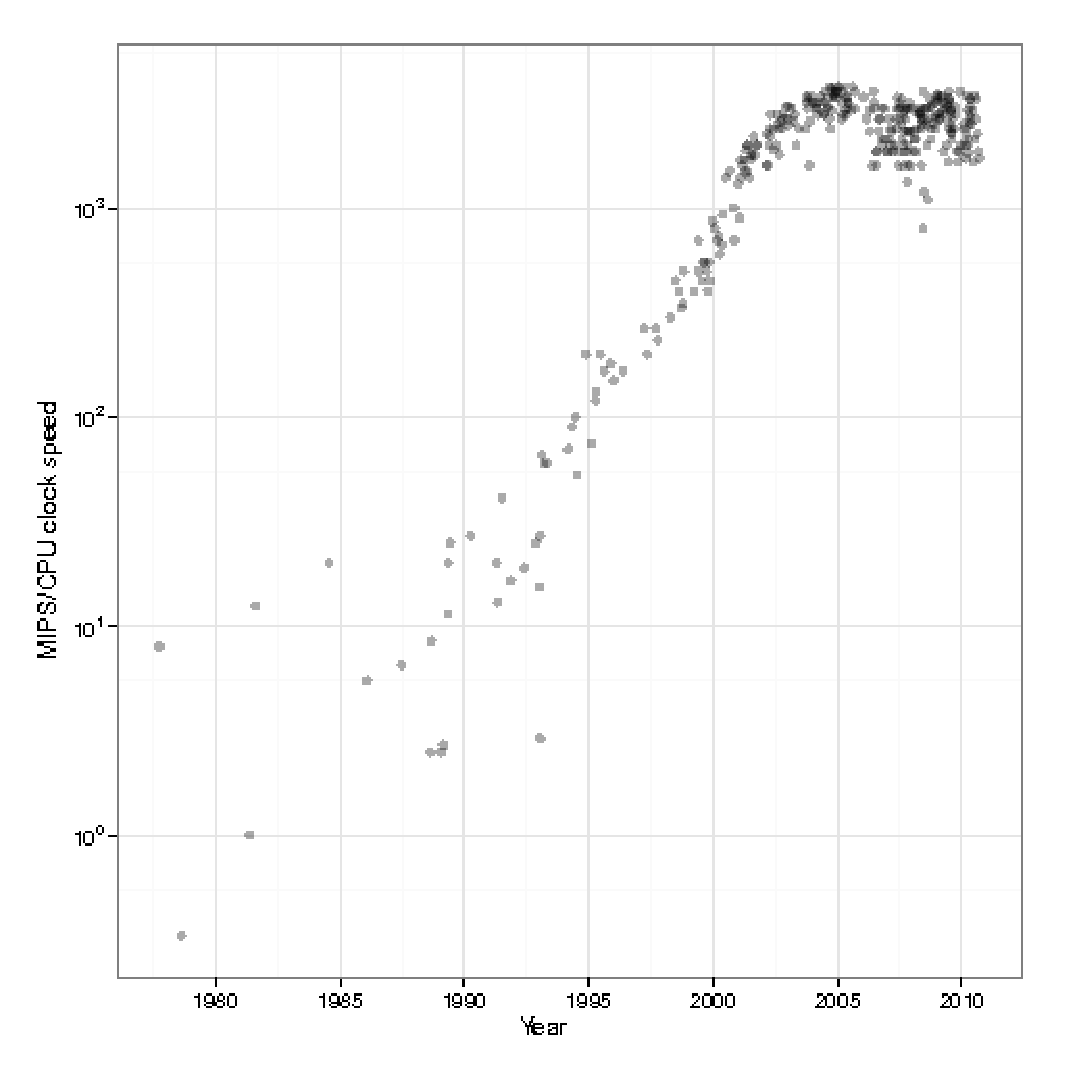
\includegraphics[width=0.5\textwidth]{cpu_and_gpu_trends}
  \caption{Evolutia puterii de procesare\cite{cpu_and_gpu_trends} }
  \label{fig:cpu_and_gpu_trends}
\end{figure}

\begin{figure}
  \centering
  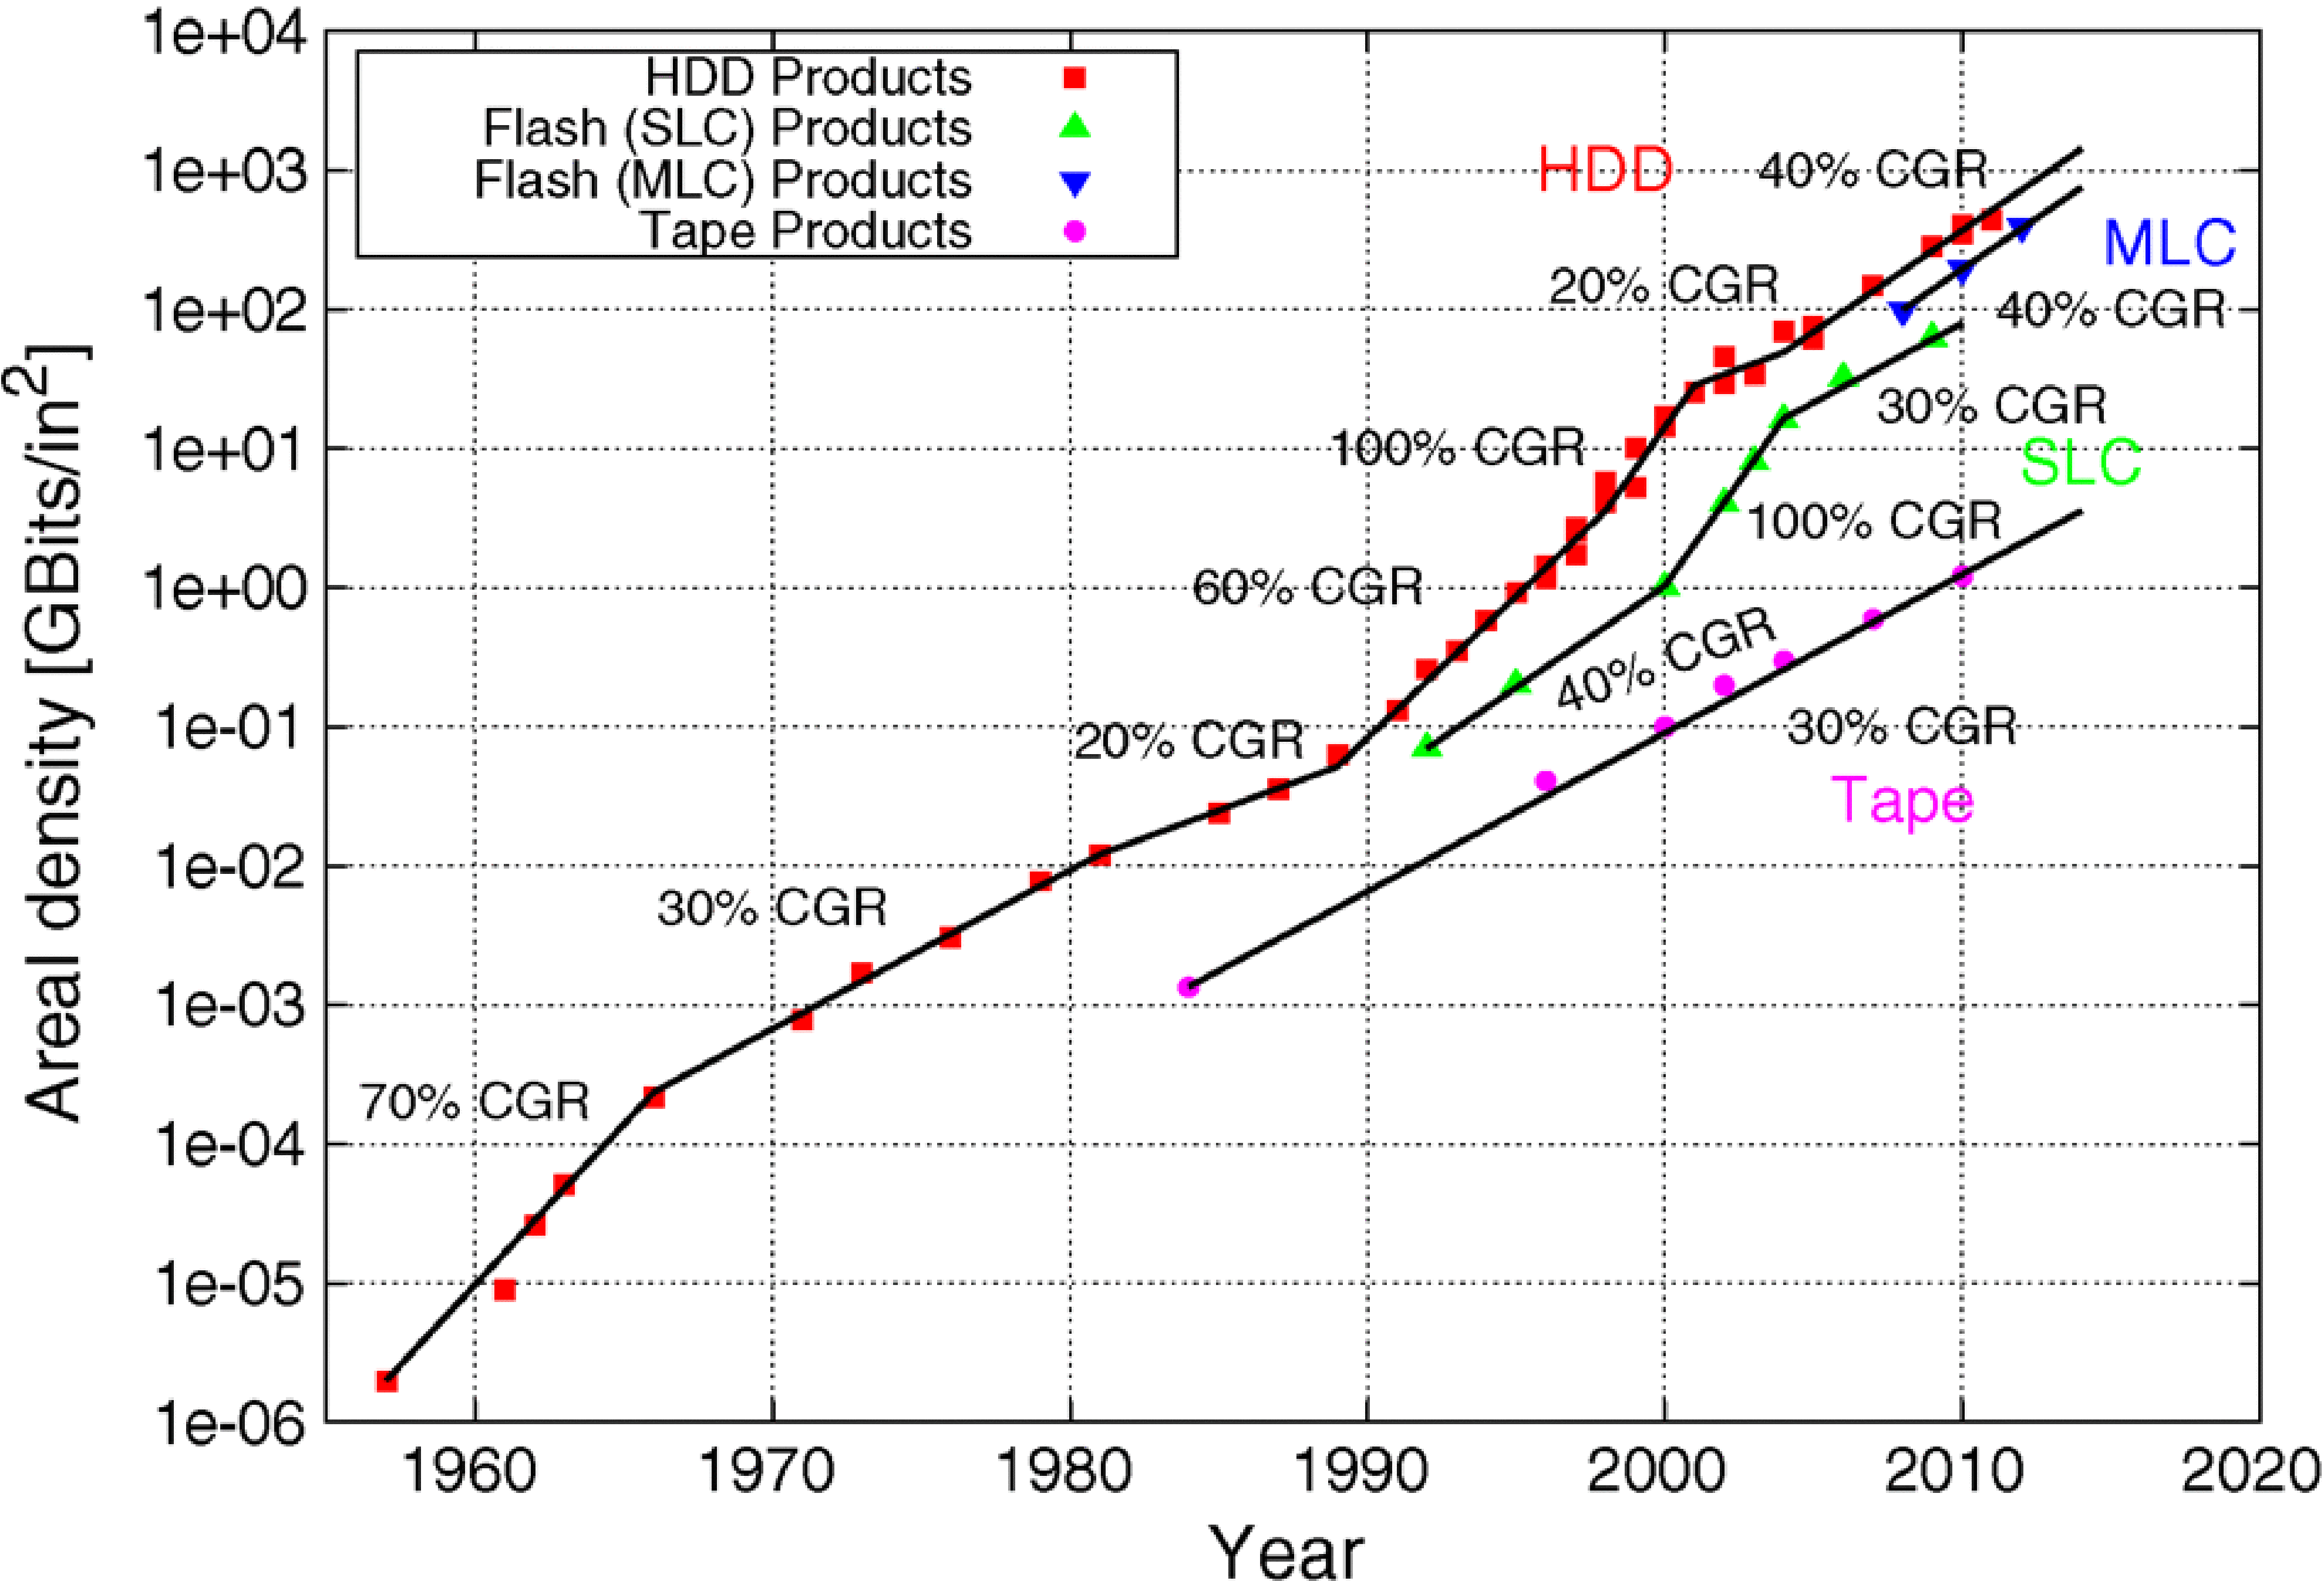
\includegraphics[width=0.5\textwidth]{memory_trends}
  \caption{Evolutia puterii de procesare\cite{memory_trends} }
  \label{fig:memory_trends}
\end{figure}

\section{Eliminarea functiilor nefolosite}

Eliminarea functiilor nefolosite este un mod de a reduce
dimensiunea programelor.

TODO(ericpts): continue
